\documentclass[14pt,a4paper]{article}
\usepackage[14pt]{extsizes}
\usepackage[left=1.5cm, right=1.5cm, top=1.5cm, bottom=1.5cm]{geometry}
\usepackage[utf8]{inputenc}
\usepackage[T2A]{fontenc}
\usepackage[english, russian]{babel}
\usepackage{amsmath,amsfonts,amssymb,amsthm,mathtools} 
\usepackage{amsfonts}
\usepackage{amssymb}
\usepackage{titleps}
\usepackage{hyperref}
\usepackage{float}
\usepackage{graphicx}
\usepackage{multirow}
\usepackage{hhline}
\usepackage{wrapfig}
\usepackage{tikz}
\usepackage{pgfplots}
\usepackage{xcolor}
\usepackage{subfig}
\usepackage{upgreek}

\newcommand{\w}[1]{\text{#1}}
\newcommand{\und}[1]{\underline{#1}}
\newcommand{\img}[3]{
	\begin{figure}[H]
	\begin{center}
	\includegraphics[scale=#2]{#1}
	\end{center}
	\begin{center}
 	\textit{#3}
	\end{center}
	\end{figure}
}
\newcommand{\aw}[1]{
	\begin{center}
	\textit{#1}
	\end{center}
	\n
}
\newcommand{\be}[1]{
	\begin{center}
	\boxed{#1}
	\end{center}
}
\newcommand{\beb}[1]{
	\begin{equation}
	\boxed{#1}
	\end{equation}
}
\newcommand{\eb}[1]{
	\begin{equation}
	#1
	\end{equation}
}
\newcommand{\n}{\hfill \break}
\newcommand{\x}{\cdot}

\begin{filecontents*}{data.csv}
\end{filecontents*}

\begin{document}

\section*{Работа 3.4.5}	
\section*{Петля гистерезиса (динамический метод)}
\subsection*{Киркича Андрей, Б01-202, МФТИ}

\section*{Экспериментальная установка}

\textbf{В работе используются:} понижающий трансформатор, реостат, резистор, интегрируюшая цепочка, амперметр и вольтметр (мультиметры), электронный осциллограф, делитель напряжения, переключатель, тороидальные образцы с двумя обмотками.
\n\n
Схема установки представлена ниже. Напряжение сети через разделительный понижающий трансформатор Тр. подаётся на намагничивающую обмотку $N_0$ образца. Значение тока в обмотке измеряется амперметром А, с ним последовательно подключено сопротивление $R_0$, напряжение с которого подаётся на вход Х электронного осциллографа ЭО. Это напряжение пропорционально току в обмотке $N_0$, а значит и напряжённости магнитного поля $H$ в образце.\n

\begin{center}
    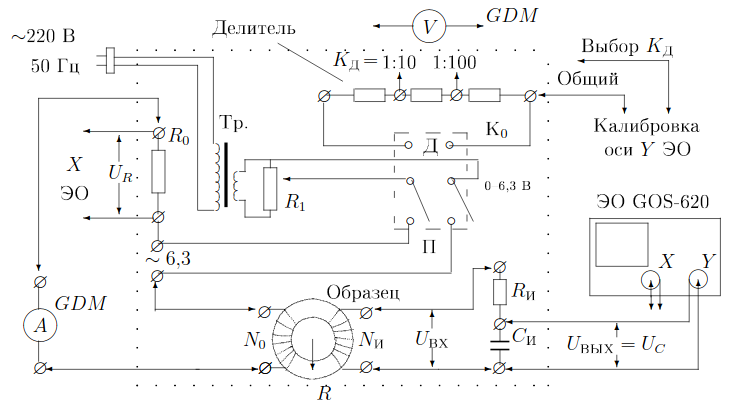
\includegraphics[width=0.9\textwidth]{1.png}
    \label{pic1}
\end{center}

\n
Для измерения магнитной индукции $B$ с измерительной обмотки $N_{\text {И }}$ на вход интегрируюшей RC-цепочки подаётся напряжение $U_{\mathrm{BX}},$ пропорциональное производной $\frac{dB}{dt},$ a $\mathrm{c}$ выхода снимается напряжение $U_{\text{BЫX}}=U_{C},$ пропорциональное величине $B,$ и подаётся на вход $Y$ электронного осциллографа.

\section*{Обработка результатов измерений}
%\subsection*{Калибровка}
%\begin{wrapfigure}{l}{0.5\textwidth}
%\vspace{-0.5cm}
%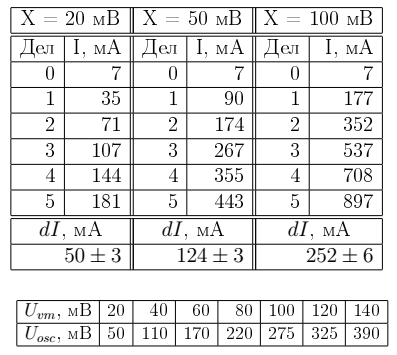
\includegraphics[scale=2.6]{2.png}
%\end{wrapfigure}
%Был откалиброван канал Х осциллографа, измерена зависимость показаний последнего от тока через амперметр. Результаты представлены в таблице. Рассчитаны коэффициенты пересчета делений в ток $dI$ для всех диапазонов.
%\n\n
%Затем был откалиброван канал Y осциллографа. Мы сравнили показания вольтметра и осциллографа и результаты занесли в таблицу. Домножив $U$ на $2\sqrt{2}$, получили, что в среднем  $U_{vm}$ отличается от $U_{osc}$ на $2$\%.
%\n

\subsection*{Изучение петель гистерезиса}

С помощью автотрансформатора были подобраны коэффициенты усиления осциллографа и ток питания в намагничивающей обмотке таким образом, чтобы предельная петля гистерезиса занимала большую часть экрана. Характеристики катушек разных материалов представлены в таблице ниже.
\begin{wrapfigure}{l}{0.6\textwidth}
	\begin{tabular}{|l|r|r|r|r|}
		\hline
		Материал     & $N_0$ & $N_\text{и}$ & $S$, см$^2$ & $2\pi R$, см \\ \hline
		Феррит       & 40    & 400                              & 3,0           & 25,0         \\ \hline
		Пермаллой    & 20    & 300                              & 0,8           & 13,3         \\ \hline
		Крем. железо & 25    & 250                              & 2,0           & 11,0         \\ \hline
	\end{tabular}
	\label{tab:har_kat}
\end{wrapfigure}
Для каждого образца мы получили передельные петли гистерезиса, по коэффициентам усиления $K_x$ и $K_y$ рассчитали масштабы, определили двойные амплитуды коэрцетивной силы $ [2x(c)] $ и индукции насыщения $ [2y(s)] $. Масштабы по осям $ X $ и $ Y $ рассчитаны по формулам:
\[ H=IN_0/(2\pi R), \qquad B=R_\text{и}C_\text{и}U_{\text{вых}}/(SN_\text{и}), \] где $I=K_x/R_0$, $U_{\text{вых}}=K_y$. Результаты измерений и вычислений представлены в таблице ниже. 

\begin{table}[H]
	\centering
	\resizebox{\textwidth}{!}{
	\begin{tabular}{|l|r|r|r|r|r|r|r|}
		\hline
		Материал     & $[2x(c)]$, дел & $[2y(s)]$, дел & $K_x, \frac{\text{мВ}}{\text{дел}}$ & $K_y, \frac{\text{мВ}}{\text{дел}}$ & $I_\text{эфф}$, мА & $H, \frac{A \x \text{м}^{-1}}{\text{дел}}$ & $B, \frac{\text{Тл}}{\text{дел}}$\\ \hline
		Феррит       & 1,0            & 4,8            & 20            & 20  & 215 & 14,5 & 0,07          \\ \hline
		Пермаллой    & 3,6            & 3,6            & 20            & 50  & 165 & 13,7 & 0,88          \\ \hline
		Крем. железо & 1,2            & 4,4            & 100           & 50  & 238 & 103,3 & 0,40          \\ \hline
	\end{tabular}
	}
\end{table}

\begin{wrapfigure}{l}{0.7\textwidth}
\vspace{0.3cm}
\resizebox{0.7\textwidth}{!}{
	\begin{tabular}{|l|r|r|r|r|}
		\hline
		Материал     & $H_c$, А/м & $B_s$, Тл & $H_{c}^{\text{теор}}$, А/м & $B_{s}^{\text{теор}}$, Тл \\ \hline
		Феррит       & $7,3 \pm 0,8$                & $0,16 \pm 0,01$ & 20 & 0,27              \\ \hline
		Пермаллой    & $24,6 \pm 2,2$                & $1,58 \pm 0,13$ & 11--40 & 1,51              \\ \hline
		Крем. железо & $62,0 \pm 7,3$                & $0,88 \pm 0,06$ & 50--100 & 1,21              \\ \hline
	\end{tabular}
	}
\end{wrapfigure}
\n
Зная масштабы по осям, можно определить значения коэрцетивной силы $ H_c $
и индукции насыщения $ B_s $. Сравнивая полученные данные с табличными можно утверждать, что они совпадают, по крайней мере, по порядку величины. Ниже приведены фотографии предельных петель гистерезиса.

\begin{figure}[H]
	\centering
	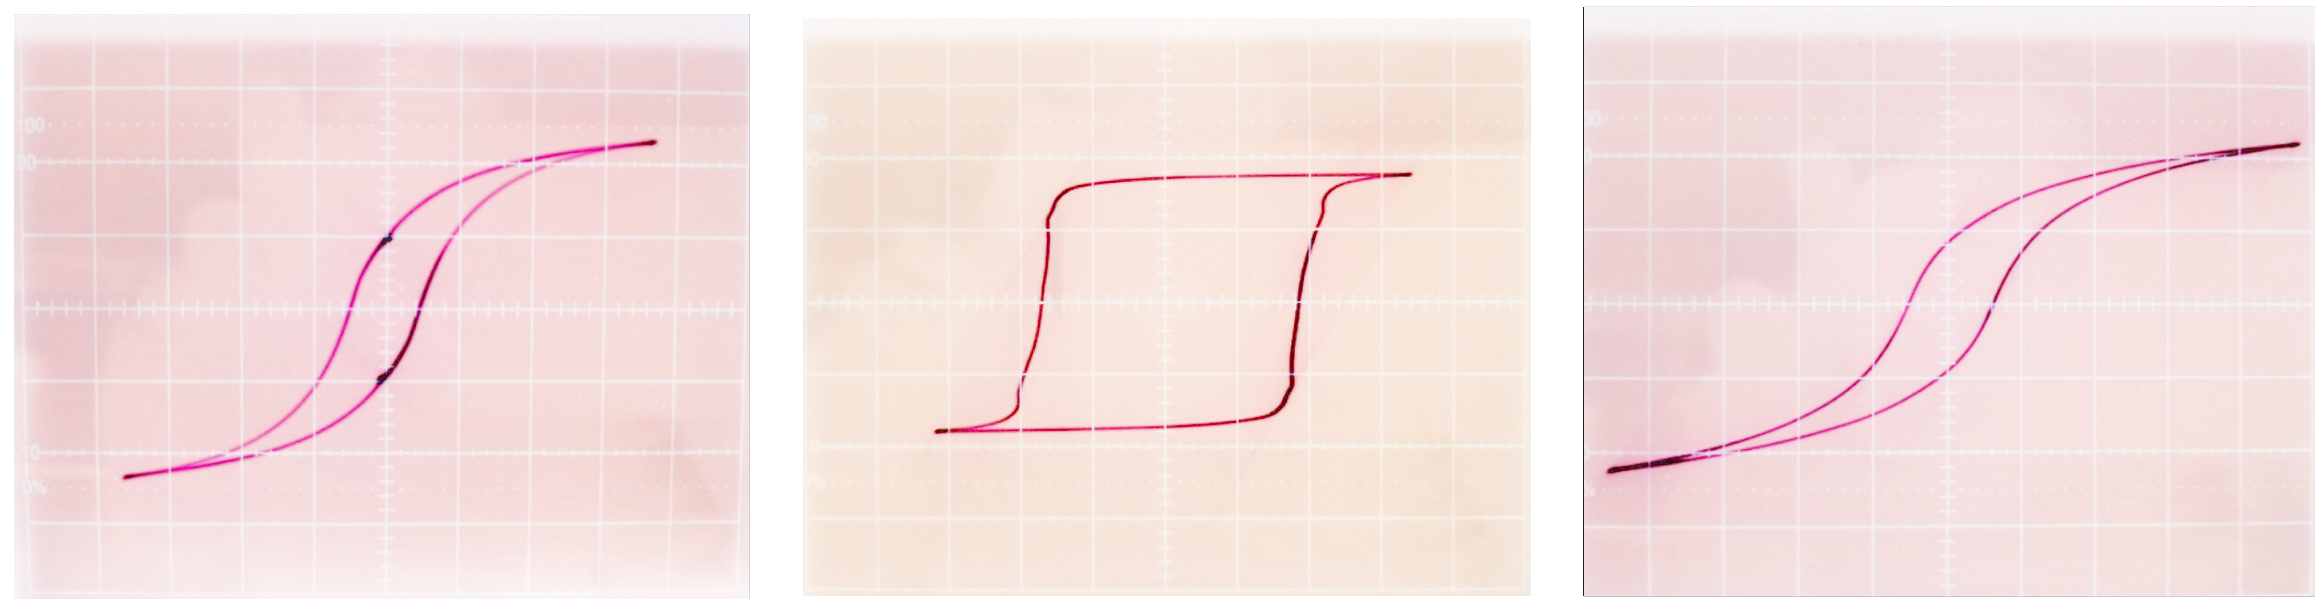
\includegraphics[width=0.9\textwidth]{3.jpg}
	\caption{Предельные петли гистерезиса феррита, пермаллоя и кремнистого железа (слева направо)}
\end{figure}

\subsection*{Проверка калибровки осциллографа}

Была проверена калибровка осциллографа по оси X. Для этого мы отключили намагничивающую обмотку $N_0$ от цепи, соединив оба провода, идущих к обмотке, на одной ее клемме. С помощью автотрансформатора был подобран такой ток через $R_0$, при котором горизонтальная прямая занимала большую часть экрана. При $ K_x=0,1 \text{ В/дел} $ была рассчиатана чувствительность $m_x=0,097 \text{ В/дел}$, аналогичные действия были проведены при $ K_x =0,02 \text{ В/дел} $. Получили $ m_x=0,019 \text{ В/дел} $.
\n\n
Так как $m_x \approx K_x$, осциллограф откалиброван по оси X корректно.
\n\n
Также нужно было проверить калибровку по оси $ Y $. Для этого мы соединили вход Y с клеммами делителя "1:100 - земля". Не меняя рабочего коэффициента $K_y = 0,05\text{ В/дел}$, подбрали с помощью трансформатора напряжение, при котором вертикальная прямая занимала большую часть экрана. Подключив вольтметр V к тем же клеммам делителя и используя измеренное $U_{\text{эф}}$, рассчитали чувствительность $m_y=0,048\text{ В/дел}$, те же действия повторили при $K_y = 0,02\text{ В/дел}$. Получили $m_y=0,017\text{ В/дел}$.
\n\n
Так как $m_y \approx K_y$, осциллограф откалиброван по оси Y корректно.

\section*{Заключение}
В ходе выполнения данной лабораторной работы были исследованы петли гистерезиса для трех различных образцов и получены характерные величины для каждого образца, которые сошлись с табличными значениями по порядку величины. Кроме того, была проверена применимость используемого метода в условиях нашего эксперимента. В итоге было установлено, что условия применимости выполняются и метод является неплохим способом определения характерных параметров для ферромагнитных материалов.

\section*{Список литературы}
1. \textit{Сивухин Д.В.} Общей курс физики. Том 3. Электричество и магнетизм, 2004\n
2. \textit{Кириченко Н.А.} Электричество и магнетизм, 2011\n
3. \textit{Максимычев А.В., Никулин М.Г.} Лабораторный практикум по общей физике. Том 2. Электричество и магнетизм.
\end{document}
